
\begin{table}[htb]
    \renewcommand{\arraystretch}{1.5}
    \begin{tabular*}{\textwidth}{|>{\columncolor{gray!15}}p{3cm}|p{17.3cm}|}
    \textbf{\large Finding} & \textbf{\large Possible determination of Apache Server version }\section*{}\addcontentsline{toc}{section}{Finding 21 - Possible determination of Apache Server version}
    \\
    Risk& Informational\\
    Category& Information Disclosure\\
    Impact& An attacker is able to see the Apache version of the service running on port 80\\\\
    Description& As shown in the graphic below the output of an nmap scan disclosed the version of the Apache server.
    \newline
    \newline
    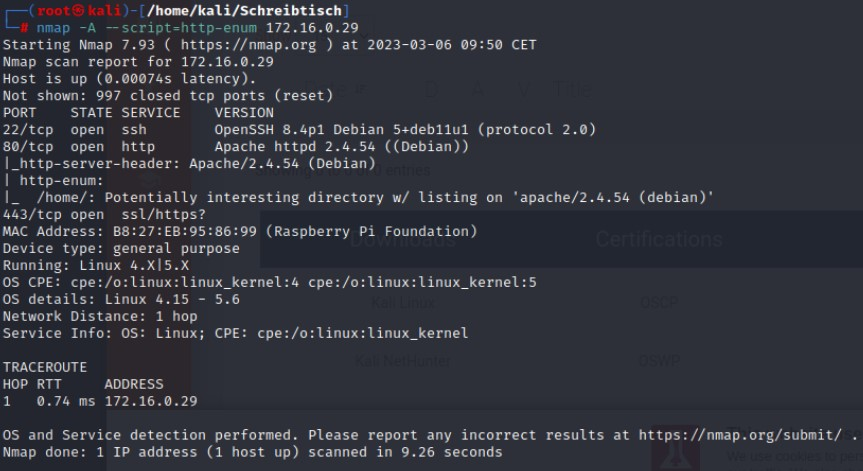
\includegraphics[width=0.85\textwidth]{http_vulnerbility.jpg}
	\\ 
	&\\
	&\\
    Recommendation& Edit the Apache Server configuration file. Change the value of ''ServerToken'' to ''Prod'' or ''ProductOnly''. This will remove the version number from the HTTP response headers and consequently the version will be hidden.\\    
    \\\\\\\\\\\\\\\\\\\\\\\\\\\\\\\\\\\\\\\\\\\\\\\\\\

    \end{tabular*}
    \end{table}